\chapter{Methods}\label{chap:methods}
% Evaluation Criteria:
% - Explanation
% - Reproducibility
% - Visualization
\todo{write methods introduction}
\draft{
Chapter on tools (language models) used. What exactly do I want to explain?
First, a bit on how they work in general, second a bit of background on the models, a bit of a comparison (architecture and benchmarks?)
}

% background is more general, methods is specific to the methods we use, in our case LLMs

\section{Language Model Basics}\label{sec:basics}
This Section aims to provide an overview of the language models used in this work as well as a fundamental understanding of the underlying concepts and terminology.
First, the fundamentals of the original transformer architecture are being established in \subref{transformer}.
\subref{modern} reintroduces the transformer architecture from a modern perspective, and highlights changes relative to the original architecture.
Last but not least, \subref{llm} provides information on the scaling up and development of modern \glspl{LLM}.

\begin{figure}[!htb]
    \begin{centering}
        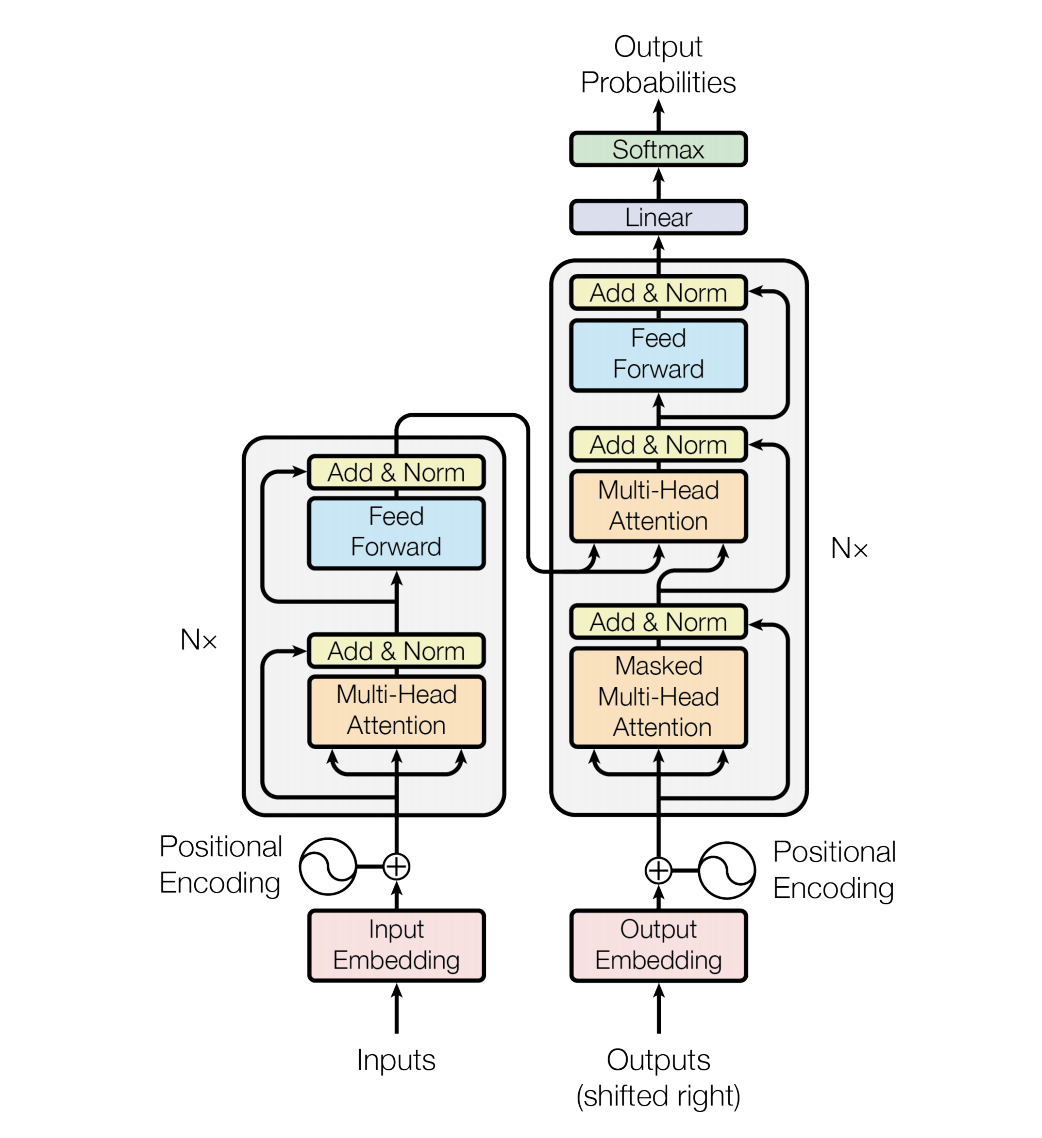
\includegraphics[height=0.5\textheight]{img/transformer}
        \caption[Original Transformer Architecture]{\textbf{Original Transformer Architecture.}
        The architecture was originally conceptualized for translation between languages.
        For that effect the text to translate (input) will be fully encoded to the embedding space, added to a positional encoding, and passed through alternating layers of self-attention and \gls{MLP} feed-forward layers with \gls{ReLU} activation, with residual connections and normalization after each.
        Output is generated autoregressively (generating each output token one-by-one, and append it to outputs to generate the next one), and has an additional layer of cross-attention to the input embedding.
        \Glspl{causal} are exclusively autoregressive decoder-only models.
        % The text to translate \textit{from} is the input, and the model will autoregressively (append selected output token to the outputs to generate the next output token until the full output has been generated) generate the full output.
        Image Source: \cite{vaswani_attention_2017}
        }
        \label{fig:transformer}
    \end{centering}
\end{figure}

% \begin{figure}[!htbp]
%     \begin{centering}
%         \subfloat[Runtime in minutes for correcting 25kb Matrix]
%         {\includegraphics[scale=0.9]{figures/results/runtime_25}} \\
%         % \caption[Correction time of 25kb]
%         % {\textbf{Runtime in minutes} for correcting the 25kb matrix.}
%         \subfloat[Runtime in minutes for correcting 50kb Matrix]
%         {\includegraphics[scale=0.9]{figures/results/runtime_50}}
%         \caption[Algorithm Runtimes]
%         {\textbf{Algorithm Runtimes} for correcting the different matrices. It
%         remains an open question why the difference between KR and RUST stays the
%         same, even though both ICE and RUST double their computation time. Smaller
%         is better.}
%         \label{fig:transformer}
%     \end{centering}
% \end{figure}


\subsection{The Transformer Architecture}\label{sub:transformer}
All modern language models are based on what was introduced as the transformer architecture \cite{vaswani_attention_2017} by \gls{Google} in 2017.
This architecture was originally designed for translation, with an encoder and a decoder part (See \figref{transformer} for more details).
The text to translate is first encoded to the embedding space by the encoder, after which the decoder will autoregressively (only one token for each full forward pass, where the most recent one will be appended to the output) generate the output, token by token.

This new transformer architecture quickly established itself by outperforming other architectures available at the time with only a fraction of the training cost.
An encoder-only transformer architecture, specifically \gls{BERT}, set a new \gls{SOTA} for all \gls{NLP} benchmarks established at the time \cite{devlin_bert_2018}.
% This success was not limited to \gls{NLP} tasks.

% Along with significantly increasing capability in \acrlong{NLP}, these models enabled more sophisticated requests for data extraction.

% main difference to before: enabled more context compared to LSTM-based attention stuff (andscaling)

\subsection{A Modern Transformer Architecture}\label{sub:modern}

There have been various attempts at improving the transformer architecture, some of them more successful than others \cite{shazeer_glu_2020, su_roformer_2022, ainslie_gqa_2023, bolya_hydra_2022, sukhbaatar_adaptive_2019, lu_understanding_2019, ye_understanding_2023, wu_memorizing_2022}.
A number of these variations have been adapted, and are used when setting up a new transformer model with few exceptions.
Refer to \figref{modern_transformer} for a graphic representation and additional description.

Early transformer architectures used \gls{ReLU} as an activation function. By comparing different activation functions, it was found that \gls{SwiGLU} empirically works best in most situations. % \cite{shazeer_glu_2020}
Surprisingly, even though dropout established itself as extremely robust technique against overfitting and forcing generalization  \cite{srivastava_dropout_2014}, few modern \gls{LLM} architectures make use of it.
This may be due to a lack of available high-quality training data.

An even better overall performance was achieved when using the more sophisticated \gls{RoPE} instead of previous sinusoidal encoding for positions.
% \cite{su_roformer_2022}
Normalizing with RMSNorm as LayerNorm \cite{ba_layer_2016}, and using it before instead of after each layer resulted in less erratic training.
In addition, a further marginally improved performance and parameter count reduction could be achieved by grouping attention query heads together in \gls{GQA}.
% \cite{ainslie_gqa_2023}
% work better than no sharing or full individual heads \cite{bolya_hydra_2022}.

Because the computational complexity based on context length for the original transformer architecture is $O(n^2)$, numerous approaches attempted to improve that \cite{child_generating_2019, wu_fastformer_2021, bolya_hydra_2022, hua_transformer_2022, dao_flashattention_2022}.
Noteworthy and practically used are in particular sparse attention \cite{child_generating_2019} (in $O(n\sqrt{n})$), and FlashAttention \cite{dao_flashattention_2022}.
FlashAttention reintroduced quadratic complexity, but resolved bottlenecks in memory layout and IO throughput, achieving substantial speedups for practical sizes of context length.
Attention with linear context-length complexity has been demonstrated \cite{wu_fastformer_2021, hua_transformer_2022}, but is not without drawbacks and thus not widely used.


\begin{figure}[!htbp]
    \begin{centering}
        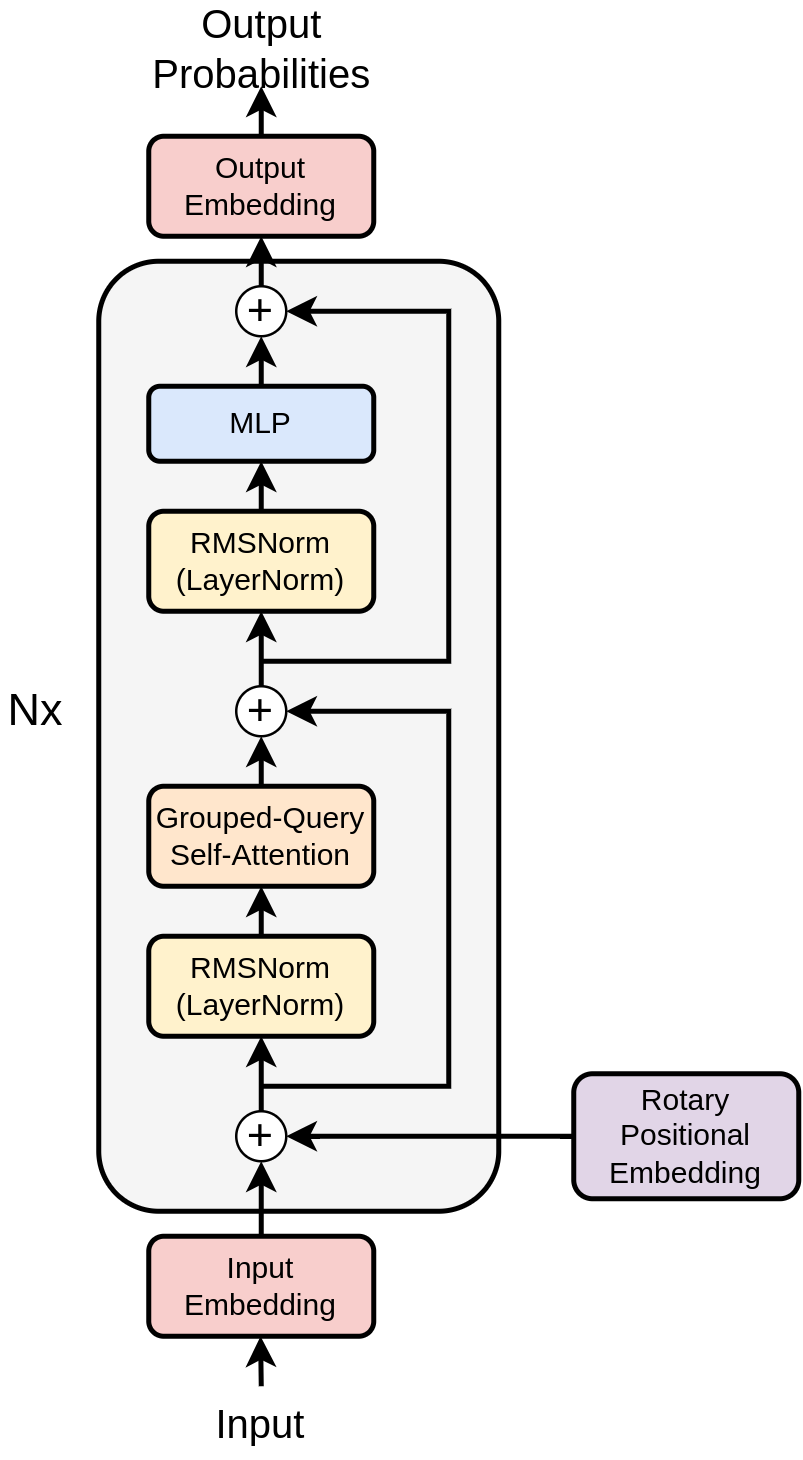
\includegraphics[height=0.8\textheight]{img/modern_transformer}
        \caption[Example of a Modern Transformer Architecture]{\textbf{Example of a Modern Transformer Architecture.} There are a number of differences when compared to the original architecture as seen previously in \figref{transformer}: layers are normalizing the residual with RMSNorm instead of having a normalized residual. Multi-head attention got replaced with \gls{GQA}, and sinusoidal positional embeddings with embeddings from \gls{RoPE} {\em on each layer}. Additionally, activation functions in the \gls{MLP} changed from \gls{ReLU} to \gls{SwiGLU}.}
        \label{fig:modern_transformer}
    \end{centering}
\end{figure}



This modern architecture as roughly described here and visualized in \figref{modern_transformer}, is used with small variations by every recent \glspl{LLM} \cite{naveed_comprehensive_2023}, and in particular those used for this work, introduced later in \secref{models}.
However, models before \model{llama2} do not use \gls{GQA}.

For a more comprehensive overview on the modern transformer architecture and modern \glspl{LLM}, refer to \cite{naveed_comprehensive_2023}.

\subsection{Large Language Models}\label{sub:llm}

\gls{GPT2} \cite{radford_language_2019} is a decoder-only \gls{LM} mostly based on the original transformer architecture, scaled up more than previous models.
Compared to other models at the time, \gls{GPT2} had up to 15x more parameters than \gls{BERT} -- 1.5 billion.
\gls{GPT2} indicated that bigger \glspl{LM} are more capable in general, only constrained by computational resources.
Models after that seem to only confirm this, and various scaling laws with diminishing returns have been observed \cite{rae_scaling_2022, hoffmann_training_2022}.
Models with multiple billion parameters became generally referred to as \acrfullpl{LLM}.

\gls{GPT3} was the first such \gls{LLM}, with 176 billion parameters, introduced by \gls{OpenAI} in 2020 \cite{brown_language_2020}.
In the months after, many more models with similar capabilities from different organizations followed.
The most well-known models of this wave were \model{BLOOM}, \model{OPT} and \gls{PaLM} \cite{chowdhery_palm_2022}.


The most recent and most capable generation of \glspl{LLM} were introduced starting early 2023, after the release of \gls{ChatGPT} sparked worldwide interest in \glspl{LLM}.
This prompted many organizations to research and advance the capabilities of \glspl{LLM}.
This renewed interest enabled fast progress in many different organizations, which culminated in dozens of advances (read more on them in \subref{modern}).

Earlier, Chinchilla \cite{hoffmann_training_2022} demonstrated that while achieving impressive capability, such large models tend to be substantially overparametrized and undertrained.
Additionally, CoTR \cite{zhang_multimodal_2023} demonstrated that existing models have not been properly utilized and are a lot more capable than previously thought.

Thus, newer models, while continuing to advance in capabilities, aren't necessarily larger.
In fact, newer models tend to be substantially more capable while being considerably smaller.
Such models include the open-access \model{llama} and its well-known derivatives \model{alpaca} and \model{vicuna}, \model{falcon}, as well as most recently \model{llama2}.

For more information on most of the aforementioned models, see the later \secref{models}.


\section{Training Large Language Models}\label{sec:training}
Training a \acrlong{LLM} heavily depends on the task the model is supposed to learn. For information on very general pretraining, see \subref{pretraining}. In \subref{finetune} additional information on fine-tuning a pretrained model is discussed. A specialized version of that, instruction-based fine-tuning is then discussed in \subref{instruct}.


\subsection{Pretraining}\label{sub:pretraining}
The objective of any \gls{causal} is to predict the next token based on the current token sequence.
Prediction of the next token only depends on previous tokens in the context.
For such scenarios, the reward is modeled as the likelihood of predicting the correct token in the sequence.
In most cases (and with few exceptions), the optimizer of choice is AdamW \cite{loshchilov_decoupled_2017}, tasked to minimize the Cross-Entropy loss of predicted tokens \cite{naveed_comprehensive_2023}.

Fully training a new model for competitive capability is a massive undertaking requiring many thousands of GPU-hours \cite{touvron_llama_2023, scao_what_2022}, with all the associated costs and carbon footprint that entails.
In order to train a \gls{LLM}, a high-quality dataset is also needed, many of which are publicly available \cite{redpajamadata_2023}.
More details on pretraining and nuances necessary for large scale distributed training can be found in \cite{tirumala_d4_2023}.
% }

\subsection{Fine-Tuning}\label{sub:finetune}
Fine-tuning exploits \textit{transfer learning} by continuing to train a previously \textit{pre-trained} model, usually with a lower training rate and on very specialized data \cite{gaddipati_comparative_2020}.
This allows \textit{transferring} previously learned features to accomplish a different task by slightly adapting the model but exploiting existing structures for feature detection.
The main benefits include using substantially less computational resources and training examples \cite{gaddipati_comparative_2020}, both of which tend to be hard to acquire, depending on the task.

As such, fine-tuning and the resulting models are usually highly specialized to their task.

\subsection{Fine-Tuning on Instructions}\label{sub:instruct}
Pre-trained or task-specific fine-tuned  models have learned context dependent token sequence likelihoods.
This is useful for predicting the 'next' token on a wikipedia article or novel, but this does not make it easy to utilize the model in other ways.

This can be solved by instead predicting the most likely token sequence when prompted with instructions instead.
Fine-tuning on instructions thus guides the output by shifting the learned context-dependent token sequence likelihood, providing more control over model outputs.
This results in users having a preference for the outputs of smaller models, over substantially bigger models, when the smaller model has been instruction fine-tuned \cite{ouyang_training_2022}, as it makes the model more `useful' in a naive sense.
A model fine-tuned on  a instruction dataset is commonly referred to as an \textit{instruct}-variant.
More details on instruction-based fine-tuning can be found in \cite{ouyang_training_2022, tirumala_d4_2023}.


% \subsection{RLHF}\label{sub:rlhf}
% learning preference policy to later fine-tune the large model on. basically lobotomization, as it drastically reduces capability.
% Well, write it a bit nicer than that.
% \todo{this is not really relevant for my thesis. remove? or write?}
